\chapter[Fundamentação Teórica]{Fundamentação Teórica}

O estudo de Inteligência Artificial vem sendo cada vez mais comum na comunidade de tecnologia da informação para a criação de sistemas que buscam automatizar e auxiliar de maneira mais eficiente o trabalho humano. O presente capítulo traz a explicação de um conjunto de tecnologias da área de IA, permitindo entender os conceitos básicos necessários para o completo entendimento da hipótese proposta.

\section{Aprendizagem de Máquina}

Aprendizado de Máquina do inglês \textit{Machine Learning} (ML) é uma das subáreas da Inteligência Artificial que visa criar mecanismos que possibilitem fazer com que uma máquina possa "aprender" sobre um determinado problema a partir de um conjunto de dados de entrada. Em outras palavras, ML permite que um dado algoritmo desenvolva uma função matemática que consiga representar tal conjunto de dados. Com essa função ou modelo matemático, é possível agora realizar inferências sobre outros dados, desde que esses sejam relacionados à mesma problemática \cite{deep-learning-book-br}.

O processo de aprendizagem se da início a partir de observações ou dados, como exemplos, experiência direta ou instruções que possibilitem identificar padrões do dado para realizar e atingir melhores decisões em futuras apresentações ou exemplos de dados que possam ser fornecidas. Dentro do processo de permitir que uma máquina aprenda, existem três áreas as quais os mecanismos de aprendizagem são classificados \cite{python-ml}:

\begin{itemize}
  \item \textbf{Aprendizado supervisionado:} o objetivo principal de algoritmos supervisionados é conseguir desenvolver um modelo matemático a partir de um conjunto de dados anotados, no caso, dados de treinamento. O \textit{supervisionado} diz respeito ao conjunto de dados os quais já se sabe a saída esperada, ou seja, o dado já é anotado previamente. Em geral, esses algoritmos são utilizados para problemas de classificação e regressão.

  % fonte: https://blogs.nvidia.com/blog/2018/08/02/supervised-unsupervised-learning/

  \begin{figure}
    \centering
    \caption{Aprendizado supervisionado}
    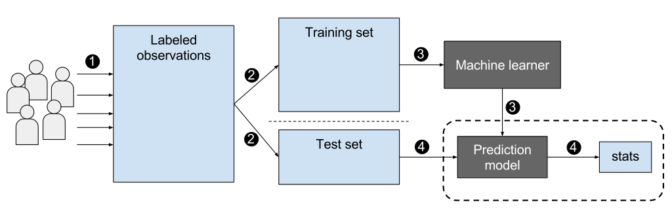
\includegraphics[scale=0.5]{figuras/nvidia-supervised-learning.png}
    \legend{Fonte: \citeonline{learning-types}}
    \label{fig:nvidia-supervised-learning}
  \end{figure}

  \newpage

  \item \textbf{Aprendizado não supervisionado:} diz respeito aos métodos de aprendizagem de máquina os quais utiliza-se como dado de entrada um dado que não possui nenhum tipo de anotação e que, muitas vezes, sua estrutura é desconhecida.

  Tal processo de aprendizagem permite extrair características relevantes sobre o dado que possam servir de insumo para uma futura categorização e classificação do mesmo. Dependendo do problema em questão, a aprendizagem supervisionada pode organizar o dado em diferentes categorias \cite{learning-types} como clusterização, associação, \textit{autoencoders}, \textit{anomaly detection}, etc.

  \item \textbf{Aprendizado semi-supervisionado:} já o aprendizado semi-supervisionado junta um pouco dos dois mundos: dados com registros anotados e também dados com registros não anotados. A aplicabilidade para esse tipo de aprendizagem é quando se possui um dado onde não é trivial extrair informações relevantes sobre ele e tampouco é realizar toda a anotação da amostra em questão \cite{learning-types}.
\end{itemize}

Dentro dos tipos de algoritmos que podem ser utilizados para construir ML, geralmente em aprendizagem supervisoonada e semi-supervisionada, um que é bastante notado se não o mais conhecido são as chamadas Redes Neurais Artificiais ou \textit{Neural Networks} (NN). Diferentemente de \textit{Machine Learning} convencional, as NN é um campo dentro de ML que possiblita o aprendizado de máquina tentando imitar o comportamento dos neurônios humanos \cite{neural-net-history} e está associado diretamente ao \textit{Deep Learning}.

\subsection{Redes Neurais}

Em 1943, Warren McCullock e Walter Pitts em seu artigo \textit{A Logical Calculus of the Ideas Immanent in Nervous Activity} desenvolveram um estudo para tentar explicar como o cérebro consegue reconhecer um nível complexo de padrões por meio dos neurônios \cite{first-neuron-study}, desenvolvendo um modelo chamado MCP (McCullock-Pitts) que atualmente é conhecido como o ancestral das redes neurais artificiais \cite{dl-brief-review}. Tal estudo possibilitou dar-se o pontapé para a evolução das redes neurais que conhecemos hoje.

Na década de 1950 surgiu então o modelo de \textit{Perceptron} \cite{perceptron}, que é a primeira rede neural formalmente desenvolvida composta de apenas uma única camada, descrito como um modelo matemático que recebe várias entradas e produz uma saída binária.

% fonte da imagem: https://towardsdatascience.com/the-perceptron-3af34c84838c

\begin{figure}[h]
  \centering
  \caption{O \textit{Perceptron}.}
  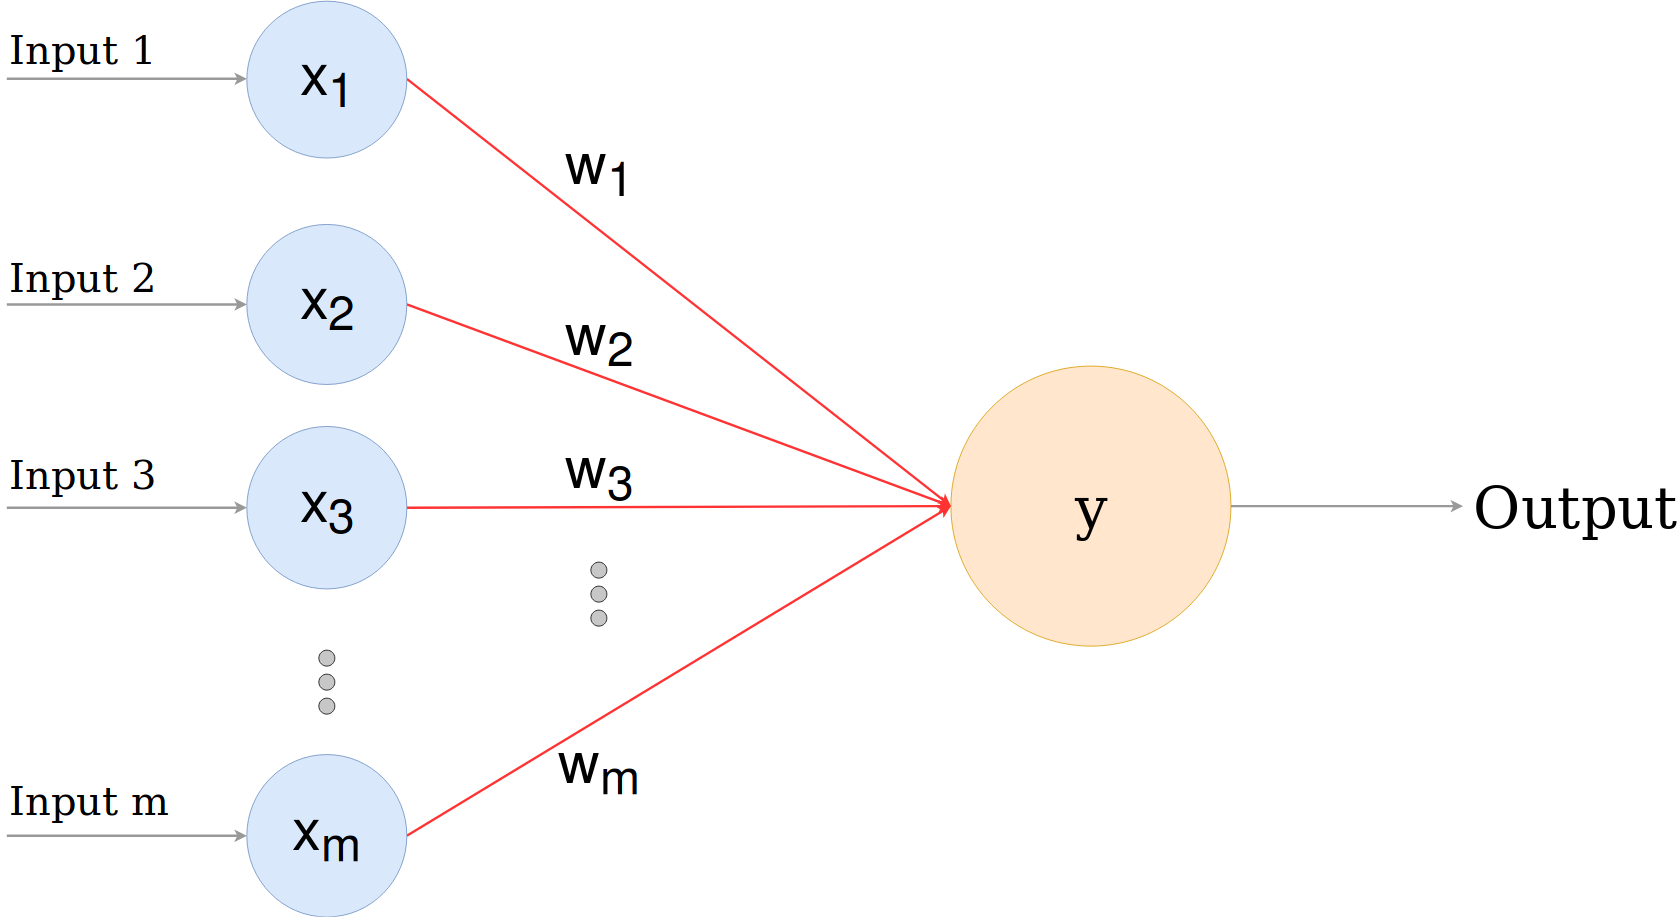
\includegraphics[scale=0.2]{figuras/perceptron}
  \legend{Fonte: \citeonline{perceptron-image}.}
  \label{fig:perceptron}
\end{figure}

Cada entrada ou \textit{input} representa um dado de entrada que é inserido diretamente nos nós de entrada ou \textit{input nodes}, representados pela letra \(x\). Cada um desses nós representam separadamente uma característica do dado de entrada. Na figura \ref{fig:perceptron}, a quantidade de características é delimitada pela letra \(m\) e o intervalo de características é dado por [1, \(m\)]. A camada caracterizada pelas letras \textit{x} é chamada de camada de entrada ou \textit{input layer}. Redes Neurais só podem receber como entrada valores numéricos \cite{deep-learning-book-br}.

É importante reparar na figura \ref{fig:perceptron} que todo nó da camada de entrada está diretamente associado com uma seta caracterizada pela letra \(w\), também de intervalo [1, \(m\)]. Tais letras caracterizam o que é conhecido como os pesos ou \textit{weights}. As setas são chamadas de sinapses\footnote
{
  Na biologia, sinapse é a região localizada entre os neurônios e agem como neurotransmissores, responsáveis por realizar a transferência de inpulso nervoso de um neurônio para o outro \cite{synapses}.
}.
Essa região é definida como camada de pesos ou \textit{weight layer}.

Por fim, tem-se o nó de maior tamanho definido pela letra \(y\), conhecido como nó de saída ou \textit{output node}. Esse nó realiza um cálculo baseado em \textit{score} sobre os valores de entrada e peso e por meio de uma função de ativação, gera uma predição \textit{output} de 0 ou 1 sobre o valor resultante do \textit{score}.

A função matemática que define o valor encontrado em \(y\) é:

\begin{gather}
  y = f(x) = \sum_{i=1}^{m} x_iw_i + B
  \label{math:perceptron-math}
\end{gather}

onde a função de ativação consome o valor resultante da função \(f(x)\), que serão melhor detalhadas na seção \ref{sssec:activation-func}. \(B\) na função define o \textit{bias} ou erro, adicionado ao valor resultante da soma de multiplicações para possíveis correções. O termo \textit{bias} foi introduzido por Tom M. Mitchell em seu artigo \textit{The Need for Biases in Learning Generalizations} \cite{biases} e o objetivo dele é possibilitar que o modelo generalize melhor o problema e seja menos sensível ao dado de entrada.

\subsubsection{Função de Ativação} \label{sssec:activation-func}

Funções de ativação são funções matemáticas que determinam o resultado de uma saída \textbf{\(z\)} de um neurônio em uma rede neural, baseando-se em um \textit{threshold}\footnote{
  Valor numérico limitante para uma tomada de ação.
} \textbf{\(t\)}.
A partir do valor resultante \textbf{\(y\)} da soma dos valores de entrada \(x_i\) multiplicados pelos pesos \(w_i\) dentro do intervalo \([1, m]\) definido na fórmula \ref{math:perceptron-math}, se esse valor alcança ou ultrapassa o \textit{threshold}, o neurônio é ativado. Caso não alcante, ele não é ativado e seu sinal não é propagado \cite{python-ml}.

\begin{gather}
  z =
  \begin{cases}
    1, & \text{se } y\geq \textit{t} \\
    0, & \text{se } y < \textit{t}
  \end{cases}
  \label{math:threshold}
\end{gather}

A função principal das funções de ativação dentro de uma rede neural é adicionar a não-linearidade ao problema, permitindo assim que tais redes consigam computar problemas não triviais \cite{gentle-intro-to-nn}. Os principais problemas que envolvem ML, principalmente no âmbito da computação visual - foco do presente trabalho -, a porcentagem de problemas que a solução é resolvida por meio de uma equação linear é praticamente - se não - zero.

Existem diversos tipos de funções de ativação com aplicabilidade em diversos tipos de problemáticas a serem resolvidas. A figura \ref{fig:activation-functions} lista as principais e mais conhecidas funções de ativação, sendo que pesquisadores ainda realizam estudos para encontrar funções que apresentem melhores resultados \cite{intro-to-act-func}.

% fonte: https://medium.com/@shrutijadon10104776/survey-on-activation-functions-for-deep-learning-9689331ba092

\begin{figure}[H]
  \centering
  \caption{Principais funções de ativação.}
  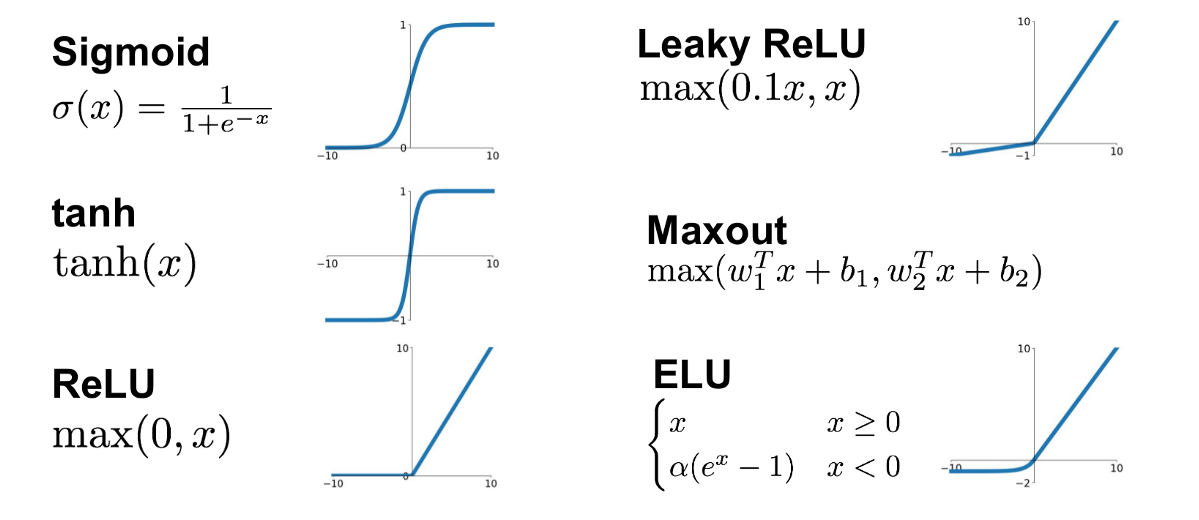
\includegraphics[scale=0.3]{figuras/activation-functions}
  \legend{Fonte: \citeonline{intro-to-act-func}.}
  \label{fig:activation-functions}
\end{figure}

É importante ressaltar que um único \textit{Perceptron} não é capaz de solucionar problemas não-lineares. Algoritmos que possibilitam solucionar problemas não-lineares serão descritos na seção \ref{sssec:cnn}, detalhando um pouco da evolução dos algoritmos para algo mais conhecido atualmente.

\subsubsection{Pesos}

Os pesos representam o grau de conexão entre dois neurônios distintos. Por exemplo: se o peso de um neurônio 1 para o neurônio 2 tem uma maior magnitude, significa que o neurônio 1 tem maior importância sobre o neurônio 2.

Em termos práticos, o peso consegue definir o quão relevante para o problema aquele determinado valor de entrada é. Pesos que se aproximam de zero tendem a diminuir a importância do valor de entrada para o valor resultante da rede \cite{everything-about-nn}.

\subsubsection{Redes Neurais Convolucionais} \label{sssec:cnn}

Conhecendo melhor o \textit{Perceptron} e entendendo como ele funciona, é possível identificar da sua limitação: a linearidade. Para solucioar esse problema, adiciona-se uma função de ativação para cada valor resultante de um nó e coloca-se esses nós em contato com mais nós de uma outra camada, adicionando assim mais camadas de processamento e identificação de características dos dados. As redes de camadas multiplas de nós ou \textit{perceptrons} é chamada de \textit{Multilayer Perceptrons} ou MLP \cite{deep-learning-book-br}.

O conjunto de de novas camadas, sendo essas diferentes da \textit{input} e \textit{output layers}, são chamadas de camadas ocultas ou \textit{hidden layers} \cite{goodfellow-et-al-2016}. A definiçãode \textit{Deep Learning} se dá pela quantidade de camadas ocultas na arquitetura da sua rede neural, sendo a MLP a "\textit{Hello World}" das arquiteturas de RNAs. Em tais redes, a saída de cada nó de uma camada da rede é utilizada como entrada para os $N$ nós presentes na camada seguinte, permitindo que os sinais ou estímulos de um neurônio artificial possa ser utilizado por toda a rede e esse valor seja propagado até a camada de saída. Tal fenômeno é chamado de \textit{propagação para a frente} ou \textit{forward-pass}. As redes neurais com essa característica recebem o nome de \textit{Feed-forward networks}.
\\
% fonte: https://www.institutodeengenharia.org.br/site/2019/04/01/nobel-da-computacao%E2%80%8B-vai-para-os-pais-do-deep-learning/

\begin{figure}[H]
  \centering
  \caption{Rede neural simples vs rede neural profunda}
  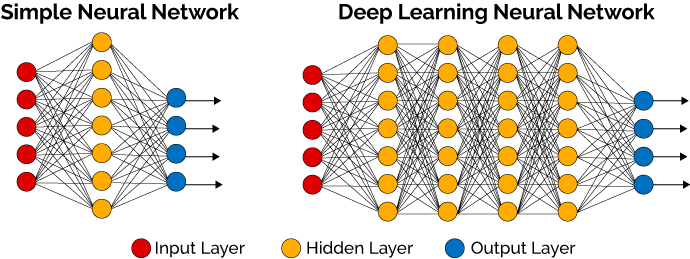
\includegraphics[scale=0.6]{figuras/simple-vs-deep-nn.png}
  \legend{Fonte: \citeonline{deep-vs-normal-net}}
  \label{fig:simple-vs-deep-nn}
\end{figure}

Mais tarde, em 1998, os pesquisadores Yann LeCun, Leon Bottou, Yosuha Bengio e Patrick Haffner desenvolveram uma nova arquitetura de rede neural herdando as características já existentes no MLP, como propagação de sinal ou \textit{forward pass}, \textit{backpropagation} (seção \ref{sssec:backpropagation}), taxa de aprendizagem, entre outros. Tal arquitetura foi chamada de LeNet-5 \cite{le-net} e sua função era conseguir reconhecer dígitos manuscritos de 0 à 9. Os dados utilizados para o experimento é chamado de \href{http://yann.lecun.com/exdb/mnist/}{MNIST}. Essa nova arquitetura evoluiu para o que conhecemos hoje como Redes Neurais Convolucionais ou CNN (\textit{Convolutional Neural Networks}) \cite{goodfellow-et-al-2016}.

\begin{figure}[H]
  \centering
  \caption{Arquitetura da LeNet-5}
  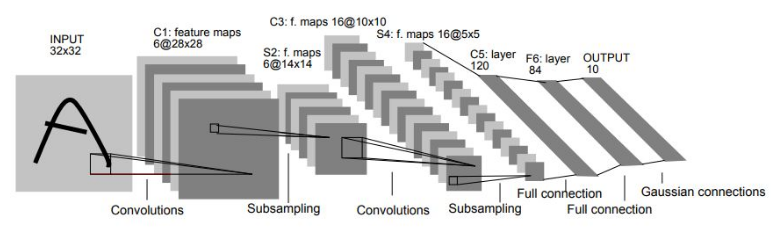
\includegraphics[width=\linewidth]{figuras/le-net.png}
  \legend{Fonte: \citeonline{le-net}}
  \label{fig:le-net}
\end{figure}

As CNNs são redes neurais especializadas em dados mais complexos, principalmente para lidar com dados de imagens \cite{goodfellow-et-al-2016}. A função da CNNs em relação a visão computacional é tentar reduzir a dimensionalidade das imagens para que o seu processamento seja mais simples, mantendo as características críticas para uma boa predição \cite{comprehensive-guide-to-cvv}.

Diferentemente das redes neurais convencionais como a MLP, as CNNs utilizam da convolução como forma de cálcular os valores dos neurons em um ou mais camadas, ao invés de utilizar cálculo matricial convencional \cite{goodfellow-et-al-2016}, e por isso herdam em seu nome a palavra \textbf{convolução}. Além disso, as CNNs utilizam possuem também, além de camadas de convolução (sessão \ref{ssssec:convolution}), camadas de \textit{pooling} (sessão \ref{ssssec:pooling}) e totalmente conectadas ou \textit{fully-connected layer}, a qual transforma o resultado das camadas de convolução e \textit{pooling} em um vetor unidimensional para que seja possível o processo de classificação que ocorre em arquiteturas de redes neurais convencionais.


\subsubsubsection{Convolução} \label{ssssec:convolution}
Na matemática, a convolução é uma operação sobre duas funções que operam com números reais (\(f\) e \(g\)) que gera uma terceira função (\(z\)) a qual expressa como uma função tende a afetar ou moldar o formato da outra. Ela representa a integral do produto de duas funções depois que uma delas foi alterada ou movida.

\begin{gather}
  z(t) = \int f(a)g(t - a) da
  \label{math:convolution}
\end{gather}

Essa é a função matemática que define a \textbf{convolução}. Para simplificação, a convolução é traduzida utilizando o símbolo de asterisco.

\begin{gather}
  z(t) = (f * g)(t)
  \label{math:convolution-simplified}
\end{gather}

Com um olhar para as redes neurais convolucionais, o primeiro argumento da convolução (\(f\)) se refere aos dados de entrada ou \textit{inputs}. O segundo argumento (\(g\)) é denominado \textit{kernel} (também chamado de filtro). O resultado (\(z\)) costuma ser referenciado como mapa de características ou \textit{feature map}. É importante ressaltar que nas CNNs, os dados presentes tanto no \textit{input} quanto os dados do \textit{kernel} devem ser números inteiros, pois trabalha-se a convolução discreta no processo matemático \cite{goodfellow-et-al-2016}.

Em aplicações de ML, o \textit{input} é geralmente tratado como um vetor multidimensional de dados e o \textit{kernel} é um vetor multidimensional de parâmetros, o qual é adaptado a medida que o processo de aprendizado corrige tais parâmetros para melhorar os resultados e minimizar a função de custo (\textit{cost function}). A função de correção dos parâmetros é chamada de \textit{backpropagation} e será tratada na sessão \ref{sssec:backpropagation}. A função de custo será tratada na sessão \ref{sssec:cost-function}.

Na prática, é possível então implementar essa integral como sendo a somatória dentro de um intervalo finito das dimensões desses vetores mutidimensionais (também chamados de tensores). Em geral, combina-se a convolução em mais de um eixo por vez sem realizar nenhum giro ou modificação em nenhuma das funções, chamando-a de correlação cruzada ou \textit{cross-relation} \cite{goodfellow-et-al-2016}, permitindo assim:

\begin{gather}
  z(i, j) = (I * K)(i, j) = \sum_{m} \sum_{n} I(i + m, j + n)K(m,n)
  \label{math:convolution-complex}
\end{gather}

Na equação \ref{math:convolution-complex} o $I$ representa o tensor de entrada, $K$ o tensor de \textit{kernel}, $i$ e $j$ a largura e altura do tensor de entrada, respectivamente, E $m$ e $n$ a largura e algura do tensor \textit{kernel}, respectivamente. Somam-se então os valores encontrados nas multiplicações a partir do tamanho do filtro e gera-se uma nova matriz com o resultado da operação. Tal matriz é a saída da camada de convolução.
\\

% a good one: https://mlnotebook.github.io/post/CNN1/
% fonte: https://medium.com/machine-learning-for-li/different-convolutional-layers-43dc146f4d0e
\begin{figure}[H]
  \centering
  \caption{Execução de uma convolução.}
  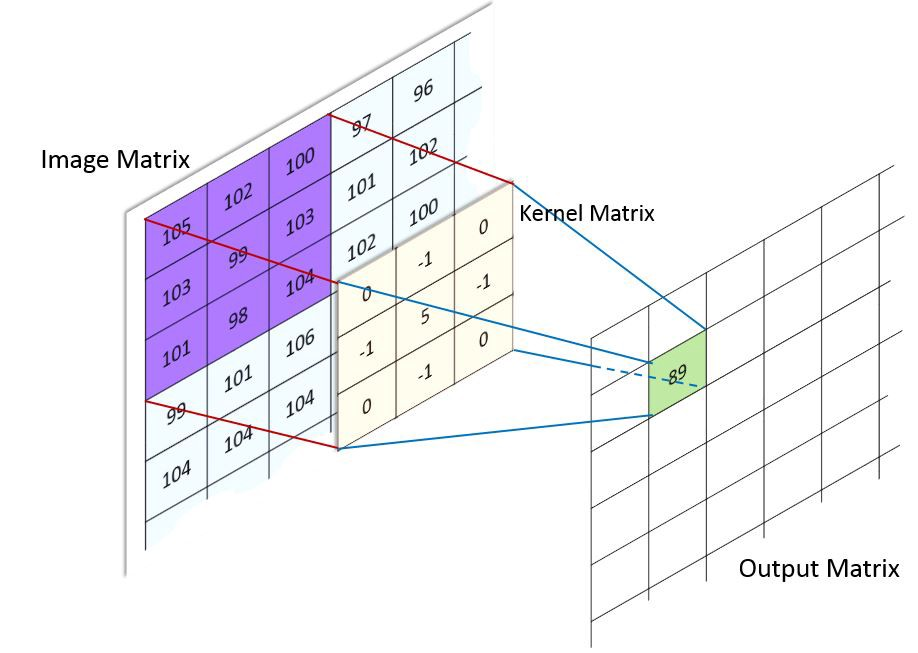
\includegraphics[scale=0.35]{figuras/cnn-kernel-multiplication.jpeg}
  \legend{Fonte: \citeonline{convolutional-medium-image}}
  \label{fig:cnn-kernel-multiplication}
\end{figure}

Existem uma série de parâmetros que podem ser utilizados para a configuração do algoritmo de convolução de uma Rede Neural Convolucional. Tais parâmetros, geralmente citados como hiperparãmetros, serão explicados de maneira geral na sessão \ref{sssec:hiperparameters}.

% O conjunto de hiperparâmetros para as CNNs, como \textit{depth}, \textit{stride}, tamanho do kernel, etc estarão melhor descritos no apêndice \hl{CRIAR APENDICE PARA REFERENCIAR}.

\subsubsubsection{\textit{Pooling}} \label{ssssec:pooling}
A operação de \textit{pooling} é utilizada geralmente após as operações na camada de convolução. Com o resultado dessa camada, algumas características são mapeadas gerando assim o \textit{feature-map} do seu dado. Com isso, com o intuito de generalizar a posição das suas características em relação a sua matriz de entrada, aplica-se o \textit{pooling} que consegue diminuir a região esparsa (geralmente com valores de pixels iguais a zero ou píxels brancos) da sua imagem, dando um foco maior para as regiões com características mais influentes para o problema.

Essa operação faz o uso de um filtro, que define o tamanho da matriz que irá percorrer os valores da matriz resultante da saída da convolução. Define-se também o \textit{stride}, que é o tamanho do passo dado a cada iteração. O resultado disso é a substituição dos valores de uma certa região (definida pelo tamanho do filtro) do resultado da camada de convolução por um valor sumarizado estatisticamente os valores dentro dessa região, definido pelo tipo de \textit{pooling utilizado}. O \textit{min-pooling} por exemplo, captura o menor falor dentro desse conjunto de valores encontrados pelo filtro, escolhe o menor valor dentre eles e mapeia para a saída da camada de \textit{pooling}.

% fonte: http://fractalytics.io/rooftop-detection-with-keras-tensorflow

\begin{figure}[H]
  \centering
  \caption{Alguns tipos de \textit{pooling}, aplicados com filtro 2x2 e passo de tamanho 2.}
  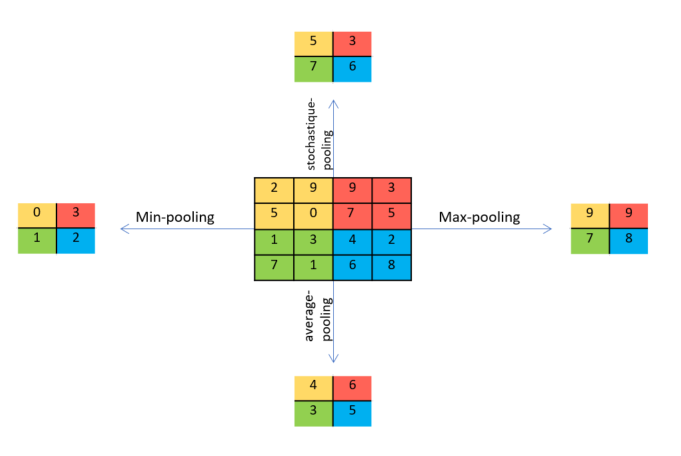
\includegraphics[width=13cm, center]{figuras/pooling.png}
  \legend{Fonte: \citeonline{pooling-types}}
  \label{fig:pooling}
\end{figure}

Em todos os casos, o \textit{pooling} auxilia em tornar a representatividade da característica mais invariantes em relação à pequenas alterações (como uma transformação, deslocamento, etc) do dado de entrada. Essa invariância significa que, independente da variação do dado, desde que pequena, o resultado da camada de \textit{pooling} não será suficientemente diferente sobre o resultado sem essa variação, permitindo uma identificação de características mais concisas. Isso pode ser útil em problemáticas cujo é importante saber se a característica está presente no dado e não o seu local exato que ela ocorre no dado, como em problemas de classificação por exemplo \cite{goodfellow-et-al-2016}.

O tamanho da matriz resultante da operação de \textit{pooling} pode ser calculada a partir da largura e altura do filtro \(L_f\) e \(A_f\), o tamanho do passo \(S\) e os tamanhos da altura e largura \(L\) e \(A\) da matriz resultante, por meio da fórmula:

\begin{gather}
  \begin{split}
    largura = \frac{L - L_f}{S}  + 1 \\
    altura =  \frac{A - A_f}{S} + 1
  \end{split}
  \label{math:size-after-pooling}
\end{gather}


\subsubsection{\textit{Backpropagation}} \label{sssec:backpropagation}

O processo o qual permite as Neural Networks aprenderem de fato é o chamado \textit{backpropagation}. Inicialmente, quando constói-se um modelo de NN para solucionar algum tipo de problemática do mundo real, inicializa-se de maneira randômica (ou seguindo algumas heurísticas) os pesos e bias da rede.

O que acontece é que nem sempre (basicamente nunca) os valores colocados inicialmente são os corretos então é preciso realizar uma alteração desses valores para permitir encontrar os pesos corretos para essas conexões. O processo que faz essa alteração é justamente o \textit{backpropagation}.

O que ela faz é basicamente calcular a derivada parcial dos pesos e biases em relação à função de erro e ajustar esses valores para que eles possam minimizar a função de custo da rede. Com isso, a medida que a rede passa por iterações no \textit{dataset}, o modelo permite se adaptar aos \textit{inputs} e conseguir gerar outputs mais aceitáveis em relação ao problema.

\begin{figure}[H]
  \centering
  \caption{Processo de \textit{backpropagation}.}
  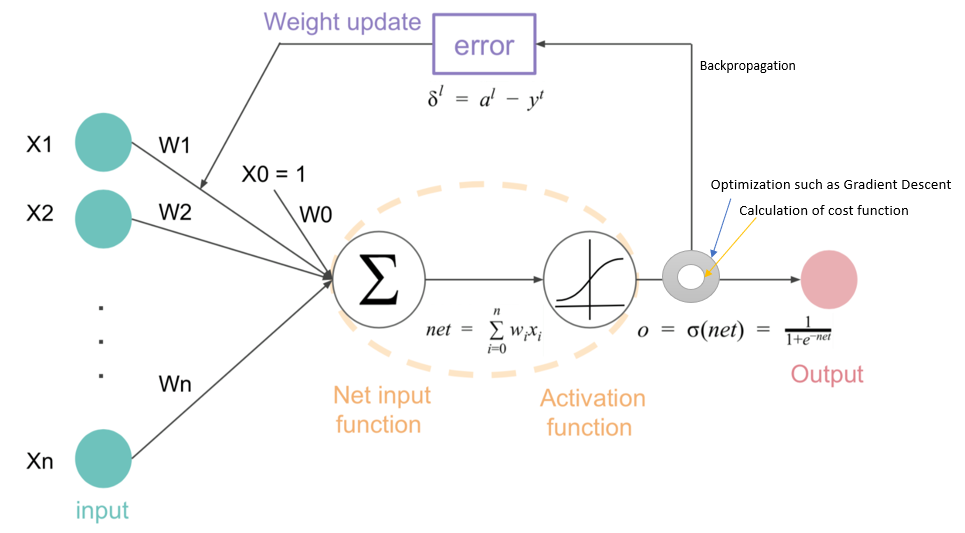
\includegraphics[scale=0.4]{figuras/backprop.png}
  \legend{Fonte: \citeonline{backprop}.}
  \label{fig:backprop}
\end{figure}

A função que permite o \textit{backpropagation} readaptar os pesos da rede é a descida de gradiente, que tende a achar a converência da função encontrando os pontos de mínima.

\begin{figure}[H]
  \centering
  \caption{Descida de gradiente.}
  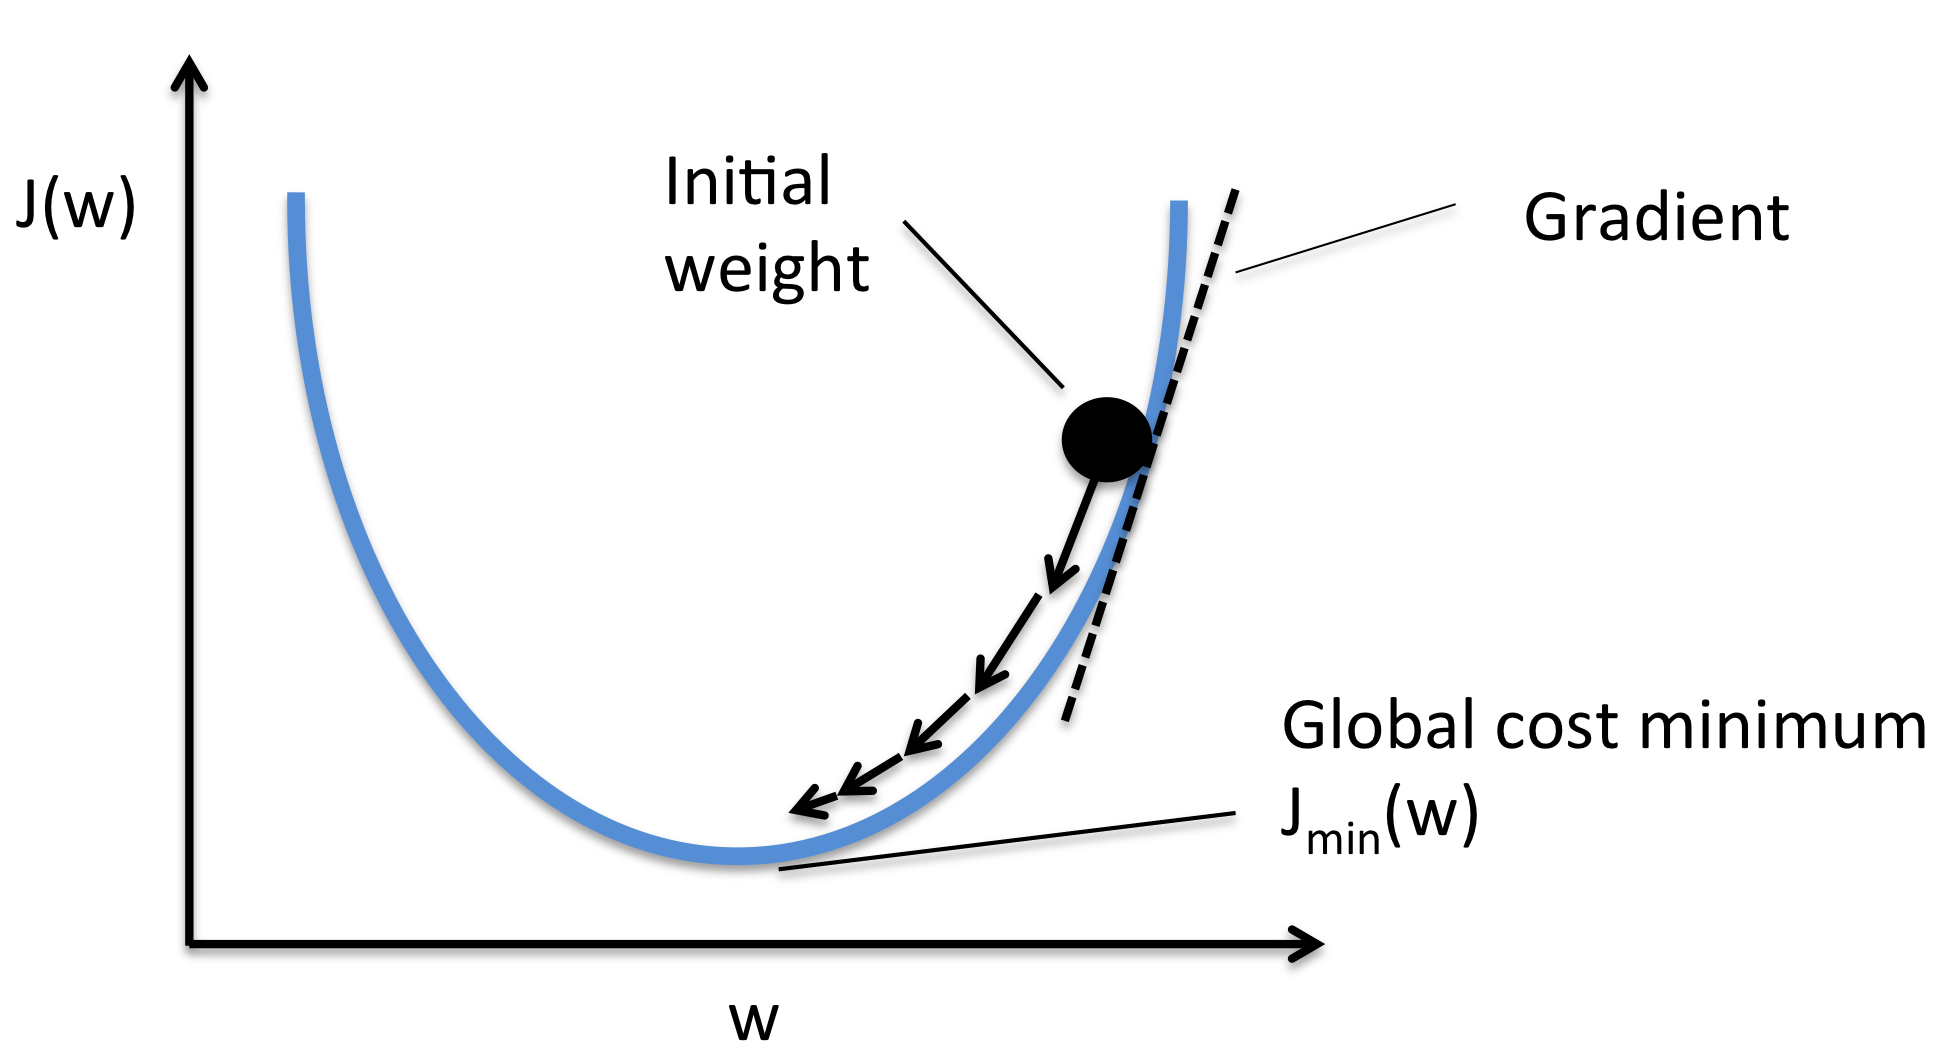
\includegraphics[scale=0.15]{figuras/gradient-descent.png}
  \legend{Fonte: \citeonline{deep-learning-book-br}}
  \label{fig:gradient-descent}
\end{figure}


\subsubsection{Função de custo ou erro} \label{sssec:cost-function}

Sabendo que é possível adequar os pesos e biases da rede neural a favor de uma progressão no problema, é preciso entender como os algoritmos conseguem identificar que estão mais próximos ou mais distantes de encontrar os valores corretos para solucionar o problema. Essa identificação é feita através da função de custo ou função de erro (do inglês \textit{cost function} e \textit{loss function}, respectivamente), a qual recebe o valor $Y_{pred}$ como resultado da rede neural sobre uma entrada de dados e o valor $Y$ esperado ou que deveria idealmente ter sido encontrado.

% https://medium.com/deep-learning-demystified/loss-functions-explained-3098e8ff2b27

\begin{figure}[H]
  \centering
  \caption{Definição de função de custo.}
  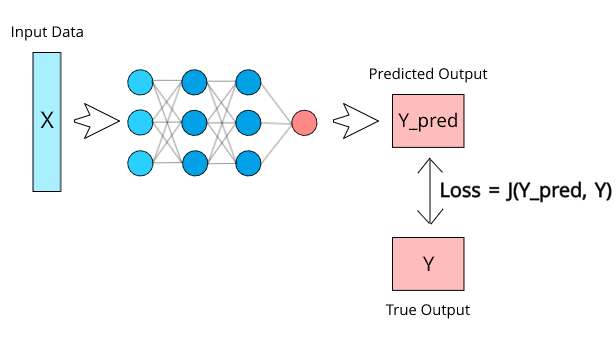
\includegraphics[scale=0.6]{figuras/cost-function.png}
  \legend{Fonte: \citeonline{cost-function}}
  \label{fig:cost-function}
\end{figure}

Essa função permite identificar o quão ruim o seu modelo está predizendo um resultado quando se comparado com o resultado correto ou o \textit{true output} na figura \ref{fig:cost-function}. Quanto mais distante o $Y_{pred}$ está do $Y$ original, mais pobre o seu resultado está sendo, então a função de custo permite penalizar o algoritmo para que ajuste os pesos necessários para tentar aproximar ambos os resultados, mostrando que o modelo está gerando saídas mais corretas e próximos ao esperado \cite{cost-function}.

\subsubsection{Hiperparâmetros} \label{sssec:hiperparameters}

Os hiperparâmetros modelam como a rede funciona e determinam sua acurácia e validade. Existem diversos métodos para otimizar os hiperparâmetros, desde modelos manuais como tentativa e erro até alguns que usam algoritmos para determinar tais alterações. Porém, não existe consenso sobre qual modelo é melhor a ser seguido na busca para achar os hiperparâmetros mais adequados.

Em uma rede, existem os parâmetros do modelo ou \textit{Model Parameters} e os \textit{Hyperparameters}. Os parâmetros do modelo são parâmetros internos à rede, como os pesos. Tais parâmetros são estimados "automaticamente" a partir das iterações de treinamento e \textit{ephocs}, e são utilizados para fazer predições no modelo. Já os hiperparâmetros são externos à rede e são definidos por quem está construindo a rede. Um bom exemplo disso é definir qual é o tipo de função de ativação a ser utilizada, o tamanho do \textit{batch} de treinamento, etc.

A alteração dos hiperparâmetros possui um enorme impacto na acurácia da rede, visto que permite adequar a rede a utilizar funções que melhor se adaptam ao tipo de dado, ao tamanho dos dados utilizados em cada \textit{ephoc} para melhorar performance, etc. A lista de alguns dos mais comuns hiperparâmetros utilizados nos processos de ajuste de rede são listados a seguir.

\begin{itemize}
  \item \textbf{Número de \textit{hidden layers}:} altera a quantidade de camadas ocultas da rede, aumentando seu nível de profundidade.
  \item \textbf{\textit{Dropout}:} define a porcentagem a qual, randomicamente, diferentes neurons da sua rede devem ser desconsiderados ou "excluídos". O uso do \textit{dropout} surge para prevenir \textit{overfitting} (modelo sabe exatamente como o dado de treimamento é mas não generaliza para dados nunca antes vistos), visto que os neurons ignorados são randômicos.
  \item \textbf{Função de ativação:} dependendo do tipo de dado a ser trabalhado, algumas funções de ativação podem não ser as mais corretas a serem utilizadas. A alteração das funções de ativação para as camadas permite que a rede possa, em certo momento, convergir para um resultado mais promissor em relação aos dados de entrada.
  \item \textbf{Inicialização de pesos:} em uma rede inicialmente não treinada, os pesos das conexões entre os neurons é totalmente desconhecido. Com isso, existe um hiperparâmetro que permite definir um modelo ou um conjunto inicial de pesos a serem utilizados na primeira iteração da rede.
  \item \textbf{\textit{Learning rate}:} taxa de aprendizagem. Em outras palavras, esse parâmetro define o quão rápido o \textit{backpropagation} está se comportando em relação à descida de gradiente, ou seja, o quão largo é o passo para encontrar os pontos de mínimo da função.
  \item \textbf{\textit{Batch size}:} dado que sua rede não é capaz de executar o \textit{epoch} com o conjunto de dados disponível, é selecionado o \textit{batch size} ou o tamanho da amostra a ser utilizado em cada \textit{epoch}.
  \item \textbf{\textit{Epochs}:} quantidade de grupo de amostras do dado que são consumidos pelo modelo por vez, excutado o \textit{backpropagation} e adaptando os pesos da rede.
  \item \textbf{Iterações:} quantidade que um único \textit{epoch} tem que ser executado para percorrer por todo o dado de treinamento, considerando também o tamanho da amostra.
  \item \textbf{Algoritmo de otimização:} é o algoritmo que de fato determina os melhores pesos do modelo. Stochastic Gradient Descent, Nesterov Accelerated Gradient, AdaDelta e Adam são os mais comuns. A otimização surge para minimizar as funções de custo do modelo.
\end{itemize}

\section{Discriminativo vs Generativo} \label{ssec:generative-vs-discriminative}

Em geral, quando ouve-se falar sobre o tema \textit{Machine Learning} naturalmente pensa-se como sendo um algoritmo que irá receber uma entrada de dados, gerar uma função matemática que se adeque aquele dado para que seja possível realizar uma classificação, seja ela binária como "Sim" \  e "Não" \  quanto uma de múltiplas categorias. Esse tipo de modelo são os chamados modelos discriminativos, que aprendem a mapear ou discriminar o dado de entrada em suas respectivas classes, ou seja, \(p(y | x)\) \cite{discriminative-vs-generative}.

\hl{CONTINUA...}

\section{\textit{Optical Character Recognition}}

Desde muitos anos, esforços e pesquisas substanciais voltadas para o reconhecimento de caracteres vêm sendo desenvolvidos, utilizados para traduzir caractéres reconhecidos por humanos para códigos interpretados pelas máquinas \cite{ocr-survey}. Mesmo para humanos, algumas vezes esse reconhecimento de caracteres não é apresentado com 100\% de acurácia, possuindo um erro de 4\% para reconhecimento de caracteres escritos à mão \cite{ocr-on-handprinted}.

O que aparenta ser uma ideia recente e inovadora, na realidade o OCR surgiu ainda na década de 20 com a ideia de máquina de leitura, proposta e patenteada por \citeonline{first-ocr-reading-machine}. O estudo de tal máquina de leitura evoluiu e se propagou pelas décadas até atingir os algoritmos que são conhecidos atualmente.

A expressão \textit{Optical Character Recognition} define uma tecnologia do ramo da computação visual capaz de receber como entrada uma imagem - necessariamente com textos - e realizar a correta identificação ou reconhecimento (\textit{recognition}) dos textos presentes na imagem \cite{ocr-survey}. Tal tecnologia deriva da capacidade humana de reconhecer e interpretar padrões presentes em um ou mais conjuntos de caracteres dos diversos alfabetos na humanidade e seus diversos formatos \cite{optical-char-recognition}. A partir dos caracteres identificados em uma image, os mesmos passam agora a ser uma mídia digital e são armazenados de uma maneira que possam ser utilizados em dispositivos informatizados.


Esse reconhecimento dos caracteres presentes na imagem é feito por diversos cálculos matemáticos para a identificação de características pertencentes a cada caracter dentro de um alfabeto. Por se tratar de um problema muito complexo e não ser o
\hl{CONTINUA...}